%% bare_conf.tex
%% V1.3
%% 2007/01/11
%% by Michael Shell
%% See:
%% http://www.michaelshell.org/
%% for current contact information.
%%
%% This is a skeleton file demonstrating the use of IEEEtran.cls
%% (requires IEEEtran.cls version 1.7 or later) with an IEEE conference paper.
%%
%% Support sites:
%% http://www.michaelshell.org/tex/ieeetran/
%% http://www.ctan.org/tex-archive/macros/latex/contrib/IEEEtran/
%% and
%% http://www.ieee.org/

%%*************************************************************************
%% Legal Notice:
%% This code is offered as-is without any warranty either expressed or
%% implied; without even the implied warranty of MERCHANTABILITY or
%% FITNESS FOR A PARTICULAR PURPOSE! 
%% User assumes all risk.
%% In no event shall IEEE or any contributor to this code be liable for
%% any damages or losses, including, but not limited to, incidental,
%% consequential, or any other damages, resulting from the use or misuse
%% of any information contained here.
%%
%% All comments are the opinions of their respective authors and are not
%% necessarily endorsed by the IEEE.
%%
%% This work is distributed under the LaTeX Project Public License (LPPL)
%% ( http://www.latex-project.org/ ) version 1.3, and may be freely used,
%% distributed and modified. A copy of the LPPL, version 1.3, is included
%% in the base LaTeX documentation of all distributions of LaTeX released
%% 2003/12/01 or later.
%% Retain all contribution notices and credits.
%% ** Modified files should be clearly indicated as such, including  **
%% ** renaming them and changing author support contact information. **
%%
%% File list of work: IEEEtran.cls, IEEEtran_HOWTO.pdf, bare_adv.tex,
%%                    bare_conf.tex, bare_jrnl.tex, bare_jrnl_compsoc.tex
%%*************************************************************************

% *** Authors should verify (and, if needed, correct) their LaTeX system  ***
% *** with the testflow diagnostic prior to trusting their LaTeX platform ***
% *** with production work. IEEE's font choices can trigger bugs that do  ***
% *** not appear when using other class files.                            ***
% The testflow support page is at:
% http://www.michaelshell.org/tex/testflow/



% Note that the a4paper option is mainly intended so that authors in
% countries using A4 can easily print to A4 and see how their papers will
% look in print - the typesetting of the document will not typically be
% affected with changes in paper size (but the bottom and side margins will).
% Use the testflow package mentioned above to verify correct handling of
% both paper sizes by the user's LaTeX system.
%
% Also note that the "draftcls" or "draftclsnofoot", not "draft", option
% should be used if it is desired that the figures are to be displayed in
% draft mode.
%
\documentclass[10pt,final,journal,a4paper]{IEEEtran}
% Add the compsoc option for Computer Society conferences.
%
% If IEEEtran.cls has not been installed into the LaTeX system files,
% manually specify the path to it like:
% \documentclass[conference]{../sty/IEEEtran}





% Some very useful LaTeX packages include:
% (uncomment the ones you want to load)


% *** MISC UTILITY PACKAGES ***
%
%\usepackage{ifpdf}
% Heiko Oberdiek's ifpdf.sty is very useful if you need conditional
% compilation based on whether the output is pdf or dvi.
% usage:
% \ifpdf
%   % pdf code
% \else
%   % dvi code
% \fi
% The latest version of ifpdf.sty can be obtained from:
% http://www.ctan.org/tex-archive/macros/latex/contrib/oberdiek/
% Also, note that IEEEtran.cls V1.7 and later provides a builtin
% \ifCLASSINFOpdf conditional that works the same way.
% When switching from latex to pdflatex and vice-versa, the compiler may
% have to be run twice to clear warning/error messages.






% *** CITATION PACKAGES ***
%
\usepackage{cite}
% cite.sty was written by Donald Arseneau
% V1.6 and later of IEEEtran pre-defines the format of the cite.sty package
% \cite{} output to follow that of IEEE. Loading the cite package will
% result in citation numbers being automatically sorted and properly
% "compressed/ranged". e.g., [1], [9], [2], [7], [5], [6] without using
% cite.sty will become [1], [2], [5]--[7], [9] using cite.sty. cite.sty's
% \cite will automatically add leading space, if needed. Use cite.sty's
% noadjust option (cite.sty V3.8 and later) if you want to turn this off.
% cite.sty is already installed on most LaTeX systems. Be sure and use
% version 4.0 (2003-05-27) and later if using hyperref.sty. cite.sty does
% not currently provide for hyperlinked citations.
% The latest version can be obtained at:
% http://www.ctan.org/tex-archive/macros/latex/contrib/cite/
% The documentation is contained in the cite.sty file itself.






% *** GRAPHICS RELATED PACKAGES ***
%
\ifCLASSINFOpdf
  % \usepackage[pdftex]{graphicx}
  % declare the path(s) where your graphic files are
  % \graphicspath{{../pdf/}{../jpeg/}}
  % and their extensions so you won't have to specify these with
  % every instance of \includegraphics
  % \DeclareGraphicsExtensions{.pdf,.jpeg,.png}
\else
  % or other class option (dvipsone, dvipdf, if not using dvips). graphicx
  % will default to the driver specified in the system graphics.cfg if no
  % driver is specified.
  % \usepackage[dvips]{graphicx}
  % declare the path(s) where your graphic files are
  % \graphicspath{{../eps/}}
  % and their extensions so you won't have to specify these with
  % every instance of \includegraphics
  % \DeclareGraphicsExtensions{.eps}
\fi
% graphicx was written by David Carlisle and Sebastian Rahtz. It is
% required if you want graphics, photos, etc. graphicx.sty is already
% installed on most LaTeX systems. The latest version and documentation can
% be obtained at: 
% http://www.ctan.org/tex-archive/macros/latex/required/graphics/
% Another good source of documentation is "Using Imported Graphics in
% LaTeX2e" by Keith Reckdahl which can be found as epslatex.ps or
% epslatex.pdf at: http://www.ctan.org/tex-archive/info/
%
% latex, and pdflatex in dvi mode, support graphics in encapsulated
% postscript (.eps) format. pdflatex in pdf mode supports graphics
% in .pdf, .jpeg, .png and .mps (metapost) formats. Users should ensure
% that all non-photo figures use a vector format (.eps, .pdf, .mps) and
% not a bitmapped formats (.jpeg, .png). IEEE frowns on bitmapped formats
% which can result in "jaggedy"/blurry rendering of lines and letters as
% well as large increases in file sizes.
%
% You can find documentation about the pdfTeX application at:
% http://www.tug.org/applications/pdftex





% *** MATH PACKAGES ***
%
\usepackage[cmex10]{amsmath}
% A popular package from the American Mathematical Society that provides
% many useful and powerful commands for dealing with mathematics. If using
% it, be sure to load this package with the cmex10 option to ensure that
% only type 1 fonts will utilized at all point sizes. Without this option,
% it is possible that some math symbols, particularly those within
% footnotes, will be rendered in bitmap form which will result in a
% document that can not be IEEE Xplore compliant!
%
% Also, note that the amsmath package sets \interdisplaylinepenalty to 10000
% thus preventing page breaks from occurring within multiline equations. Use:
%\interdisplaylinepenalty=2500
% after loading amsmath to restore such page breaks as IEEEtran.cls normally
% does. amsmath.sty is already installed on most LaTeX systems. The latest
% version and documentation can be obtained at:
% http://www.ctan.org/tex-archive/macros/latex/required/amslatex/math/





% *** SPECIALIZED LIST PACKAGES ***
%
\usepackage{algorithmic}
% algorithmic.sty was written by Peter Williams and Rogerio Brito.
% This package provides an algorithmic environment fo describing algorithms.
% You can use the algorithmic environment in-text or within a figure
% environment to provide for a floating algorithm. Do NOT use the algorithm
% floating environment provided by algorithm.sty (by the same authors) or
% algorithm2e.sty (by Christophe Fiorio) as IEEE does not use dedicated
% algorithm float types and packages that provide these will not provide
% correct IEEE style captions. The latest version and documentation of
% algorithmic.sty can be obtained at:
% http://www.ctan.org/tex-archive/macros/latex/contrib/algorithms/
% There is also a support site at:
% http://algorithms.berlios.de/index.html
% Also of interest may be the (relatively newer and more customizable)
% algorithmicx.sty package by Szasz Janos:
% http://www.ctan.org/tex-archive/macros/latex/contrib/algorithmicx/




% *** ALIGNMENT PACKAGES ***
%
\usepackage{array}
% Frank Mittelbach's and David Carlisle's array.sty patches and improves
% the standard LaTeX2e array and tabular environments to provide better
% appearance and additional user controls. As the default LaTeX2e table
% generation code is lacking to the point of almost being broken with
% respect to the quality of the end results, all users are strongly
% advised to use an enhanced (at the very least that provided by array.sty)
% set of table tools. array.sty is already installed on most systems. The
% latest version and documentation can be obtained at:
% http://www.ctan.org/tex-archive/macros/latex/required/tools/


\usepackage{mdwmath}
\usepackage{mdwtab}
% Also highly recommended is Mark Wooding's extremely powerful MDW tools,
% especially mdwmath.sty and mdwtab.sty which are used to format equations
% and tables, respectively. The MDWtools set is already installed on most
% LaTeX systems. The lastest version and documentation is available at:
% http://www.ctan.org/tex-archive/macros/latex/contrib/mdwtools/


% IEEEtran contains the IEEEeqnarray family of commands that can be used to
% generate multiline equations as well as matrices, tables, etc., of high
% quality.


\usepackage{eqparbox}
% Also of notable interest is Scott Pakin's eqparbox package for creating
% (automatically sized) equal width boxes - aka "natural width parboxes".
% Available at:
% http://www.ctan.org/tex-archive/macros/latex/contrib/eqparbox/





% *** SUBFIGURE PACKAGES ***
%\usepackage[tight,footnotesize]{subfigure}
% subfigure.sty was written by Steven Douglas Cochran. This package makes it
% easy to put subfigures in your figures. e.g., "Figure 1a and 1b". For IEEE
% work, it is a good idea to load it with the tight package option to reduce
% the amount of white space around the subfigures. subfigure.sty is already
% installed on most LaTeX systems. The latest version and documentation can
% be obtained at:
% http://www.ctan.org/tex-archive/obsolete/macros/latex/contrib/subfigure/
% subfigure.sty has been superceeded by subfig.sty.



%\usepackage[caption=false]{caption}
%\usepackage{caption}
%\usepackage[font=footnotesize, captions=false]{subfig}
% subfig.sty, also written by Steven Douglas Cochran, is the modern
% replacement for subfigure.sty. However, subfig.sty requires and
% automatically loads Axel Sommerfeldt's caption.sty which will override
% IEEEtran.cls handling of captions and this will result in nonIEEE style
% figure/table captions. To prevent this problem, be sure and preload
% caption.sty with its "caption=false" package option. This is will preserve
% IEEEtran.cls handing of captions. Version 1.3 (2005/06/28) and later 
% (recommended due to many improvements over 1.2) of subfig.sty supports
% the caption=false option directly:
%\usepackage[caption=false,font=footnotesize]{subfig}
%
% The latest version and documentation can be obtained at:
% http://www.ctan.org/tex-archive/macros/latex/contrib/subfig/
% The latest version and documentation of caption.sty can be obtained at:
% http://www.ctan.org/tex-archive/macros/latex/contrib/caption/




% *** FLOAT PACKAGES ***
%
\usepackage{fixltx2e}
% fixltx2e, the successor to the earlier fix2col.sty, was written by
% Frank Mittelbach and David Carlisle. This package corrects a few problems
% in the LaTeX2e kernel, the most notable of which is that in current
% LaTeX2e releases, the ordering of single and double column floats is not
% guaranteed to be preserved. Thus, an unpatched LaTeX2e can allow a
% single column figure to be placed prior to an earlier double column
% figure. The latest version and documentation can be found at:
% http://www.ctan.org/tex-archive/macros/latex/base/



%\usepackage{stfloats}
% stfloats.sty was written by Sigitas Tolusis. This package gives LaTeX2e
% the ability to do double column floats at the bottom of the page as well
% as the top. (e.g., "\begin{figure*}[!b]" is not normally possible in
% LaTeX2e). It also provides a command:
%\fnbelowfloat
% to enable the placement of footnotes below bottom floats (the standard
% LaTeX2e kernel puts them above bottom floats). This is an invasive package
% which rewrites many portions of the LaTeX2e float routines. It may not work
% with other packages that modify the LaTeX2e float routines. The latest
% version and documentation can be obtained at:
% http://www.ctan.org/tex-archive/macros/latex/contrib/sttools/
% Documentation is contained in the stfloats.sty comments as well as in the
% presfull.pdf file. Do not use the stfloats baselinefloat ability as IEEE
% does not allow \baselineskip to stretch. Authors submitting work to the
% IEEE should note that IEEE rarely uses double column equations and
% that authors should try to avoid such use. Do not be tempted to use the
% cuted.sty or midfloat.sty packages (also by Sigitas Tolusis) as IEEE does
% not format its papers in such ways.





% *** PDF, URL AND HYPERLINK PACKAGES ***
%
\usepackage{url}
% url.sty was written by Donald Arseneau. It provides better support for
% handling and breaking URLs. url.sty is already installed on most LaTeX
% systems. The latest version can be obtained at:
% http://www.ctan.org/tex-archive/macros/latex/contrib/misc/
% Read the url.sty source comments for usage information. Basically,
% \url{my_url_here}.

\usepackage{epsfig}
\usepackage{graphicx}
%\usepackage{subfloat}
%\usepackage{subcaption}
\usepackage[T1]{fontenc}
\usepackage{mwe}
\usepackage{subfig}
\usepackage{float}
%\usepackage{subfloat}
%\usepackage[section]{placeins}

% *** Do not adjust lengths that control margins, column widths, etc. ***
% *** Do not use packages that alter fonts (such as pslatex).         ***
% There should be no need to do such things with IEEEtran.cls V1.6 and later.
% (Unless specifically asked to do so by the journal or conference you plan
% to submit to, of course. )


% correct bad hyphenation here
\hyphenation{op-tical net-works semi-conduc-tor}


\begin{document}
%
% paper title
% can use linebreaks \\ within to get better formatting as desired
\title{Peer-Assisted Content Distribution Aided by Video Popularity Evolution Model}

\author{\IEEEauthorblockN{Mohamad Dikshie Fauzie\IEEEauthorrefmark{1} \quad
Achmad Husni Thamrin\IEEEauthorrefmark{1} \quad
Jun Murai\IEEEauthorrefmark{2}}
\IEEEauthorblockA{\IEEEauthorrefmark{1}Graduate School of Media and Governance} \quad
\IEEEauthorblockA{\IEEEauthorrefmark{2}Faculty of Environment and Information Studies\\ 
Keio University, 252-0882 Kanagawa, Japan \\
dikshie@sfc.wide.ad.jp \quad\quad husni@ai3.net \quad\quad jun@wide.ad.jp}
}




% use for special paper notices
%\IEEEspecialpapernotice{(Invited Paper)}




% make the title area
\maketitle


\begin{abstract}
%\boldmath
Generally content distribution network (CDN) have adopted two different architectures: client-server model that's is the most common architecture model and peer-assisted CDN.  
In client-server model, clients download content dedicated and geographically managed servers while in peer-assisted model, clients download part of content from each other client besides from CDN servers. 
In this paper, we develop a peer-assisted CDN model based on previous work. 
Our model is quite different from previous work.  
We add Youtube VoD views popularity model aspect to our peer-assisted CDN model. 
From simulation-based experiments driven by real-world Youtube datasets, we find that peers in our model can contribute to deliver contents higher than previous work on the other hand number of access to cache in peer also higher than previous work.
We do significance test for both metrics (peer contributions and number of access to cache) and find that $p$-values are less than $1$\% thus the results are significant.

\end{abstract}
% IEEEtran.cls defaults to using nonbold math in the Abstract.
% This preserves the distinction between vectors and scalars. However,
% if the conference you are submitting to favors bold math in the abstract,
% then you can use LaTeX's standard command \boldmath at the very start
% of the abstract to achieve this. Many IEEE journals/conferences frown on
% math in the abstract anyway.

% no keywords
\begin{IEEEkeywords}
Internet Video on Demand (VoD), P2P, CDN, and Caching.
\end{IEEEkeywords}





% For peer review papers, you can put extra information on the cover
% page as needed:
% \ifCLASSOPTIONpeerreview
% \begin{center} \bfseries EDICS Category: 3-BBND \end{center}
% \fi
%
% For peerreview papers, this IEEEtran command inserts a page break and
% creates the second title. It will be ignored for other modes.
%\IEEEpeerreviewmaketitle



\section{Introduction}
Streaming content, especially video, represents a significant fraction of the traffic volume on the Internet, and it has become a standard practice to deliver this type of content using Content Delivery Networks (CDNs) such as Akamai and Limelight for better scaling and quality of experience for the end users. 
For example, YouTube uses Google cache and MTV uses Akamai in their operations.

With the spread of broadband Internet access at a reasonable flat monthly rate, users are connected to the Internet 24 hours a day and they can download and share multimedia content. P2P (peer to peer) applications are also widely deployed. 
In China, P2P is very popular; we see many P2P applications from China such as PPLive, PPStream, UUSe, Xunlei, etc. \cite{Vu:2010:UOC:1865106.1865115}. 
Some news broadcasters also rely on P2P technology to deliver popular live events. 
For example, CNN uses the Octoshape \cite{octoshape} solution that enables their broadcast to scale and offer good video quality as the number of users increases.

From the Internet provider point of view, the presence of so many always-on users suggests that it is possible to delegate a portion of computing, storage and networking tasks to the users, thus creating P2P networks where users can share files and multimedia content. 
Starting from file sharing protocols, P2P architectures have evolved toward video on demand and support for live events.

%A P2P based architecture usually requires a sufficient number of nodes supplying the data (seeders) to start the distribution process among the joining peers.  
%A peer usually offers a low outbound streaming rate due to the traditional asymmetrical DSL home connectivity and hence multiple peers must jointly stream contents to a requesting peer (leecher).  
%The decentralized, uncoordinated operation implies that scaling to a high number of peers comes with side effects.  
%Typical problems of a P2P streaming architecture are low stream quality with undesirable disruptions, resource unfairness due to heterogeneous peer resources, and high startup delay.  
%Moreover, current P2P applications are not aware of the underlying network and may conflict with the ISP routing policies and business model.

%A number of P2P streaming applications have been designed, analyzed and deployed, attracting a significant number of users.  
%Research studies and deployment experiences have both demonstrated that P2P is a promising solution in terms of scalability and deployment costs.  
%On the other hand, the heterogeneous nature and unstable behavior of the peers contributing bandwidth and computational resources, along with the networking issues, affect the user experience and limit the commercial success of P2P video streaming applications.
Alternatively, video contents can be efficiently distributed on services offered by managed network architectures and CDN companies.
The major issues of CDN are high deployment cost and good but not unlimited scalability in the long term.  
Given the complementary features of P2P and CDN, in recent years some hybrid solutions have been proposed and applied to the operational of CDN \cite{Huang:2008:UHC:1496046.1496064,4772628,Yin:2009:DDH:1631272.1631279} to take the best of both approaches.
In Peer assisted CDN, users can download content from CDN nodes from or other users or peers. 
A user may cache the content after download to serve requests from other users. 
Due to the complexity of the behavior of peers, the process should be done in the home gateway user where the ISP can control it.

In this work, we will revisit Guo et al., \cite{1613869} work's PROP as basis to evaluate of the peer-assisted CDN and propose an improvement the model for the PROP.
We also examine the characteristics of Internet VoD by investigating real-world datasets obtained from Youtube.
In P2P assisted CDN for video on demand (VoD), most of researcher assume that catalog of video popularity rank is already established following zipf distribution.  
This become basis for P2P assisted CDN model in PROP \cite{1613869}.
Our work is quite different whereas we will use VoD view popularity to aid the PROP model.
We use Youtube VoD view model for this purpose.
%In Youtube, video view popularity has three phase which is before-peak, at-peak, and after-peak \cite{Borghol:2011:CMP:2039452.2039717} which we will explain later in sect.\ref{popularity}.
A twofold of our contributions as follows:
(1) We use the idea of VoD view popularity model to aid the PROP model. 
To our knowledge, the combination of PROP model and VoD view popularity model is the first.
(2) From simulation-based experiments, we find that peer contributions become higher than the PROP model.

Our paper presentation as follows: (1) we describe related work in sect.\ref{relatedwork}; (2) we explain detail of Youtube popularity evolution model in sect.\ref{popularity}; (3) we explain the caching strategy for CDN and peer in sect.\ref{systemdescription}; (4) we explain our simulation design, simulator, and its evaluation in sect.\ref{evaluation}.
Finally, we present our conclusions in section \ref{conclusion}.

%\begin{figure}[!t]
%\begin{center}
%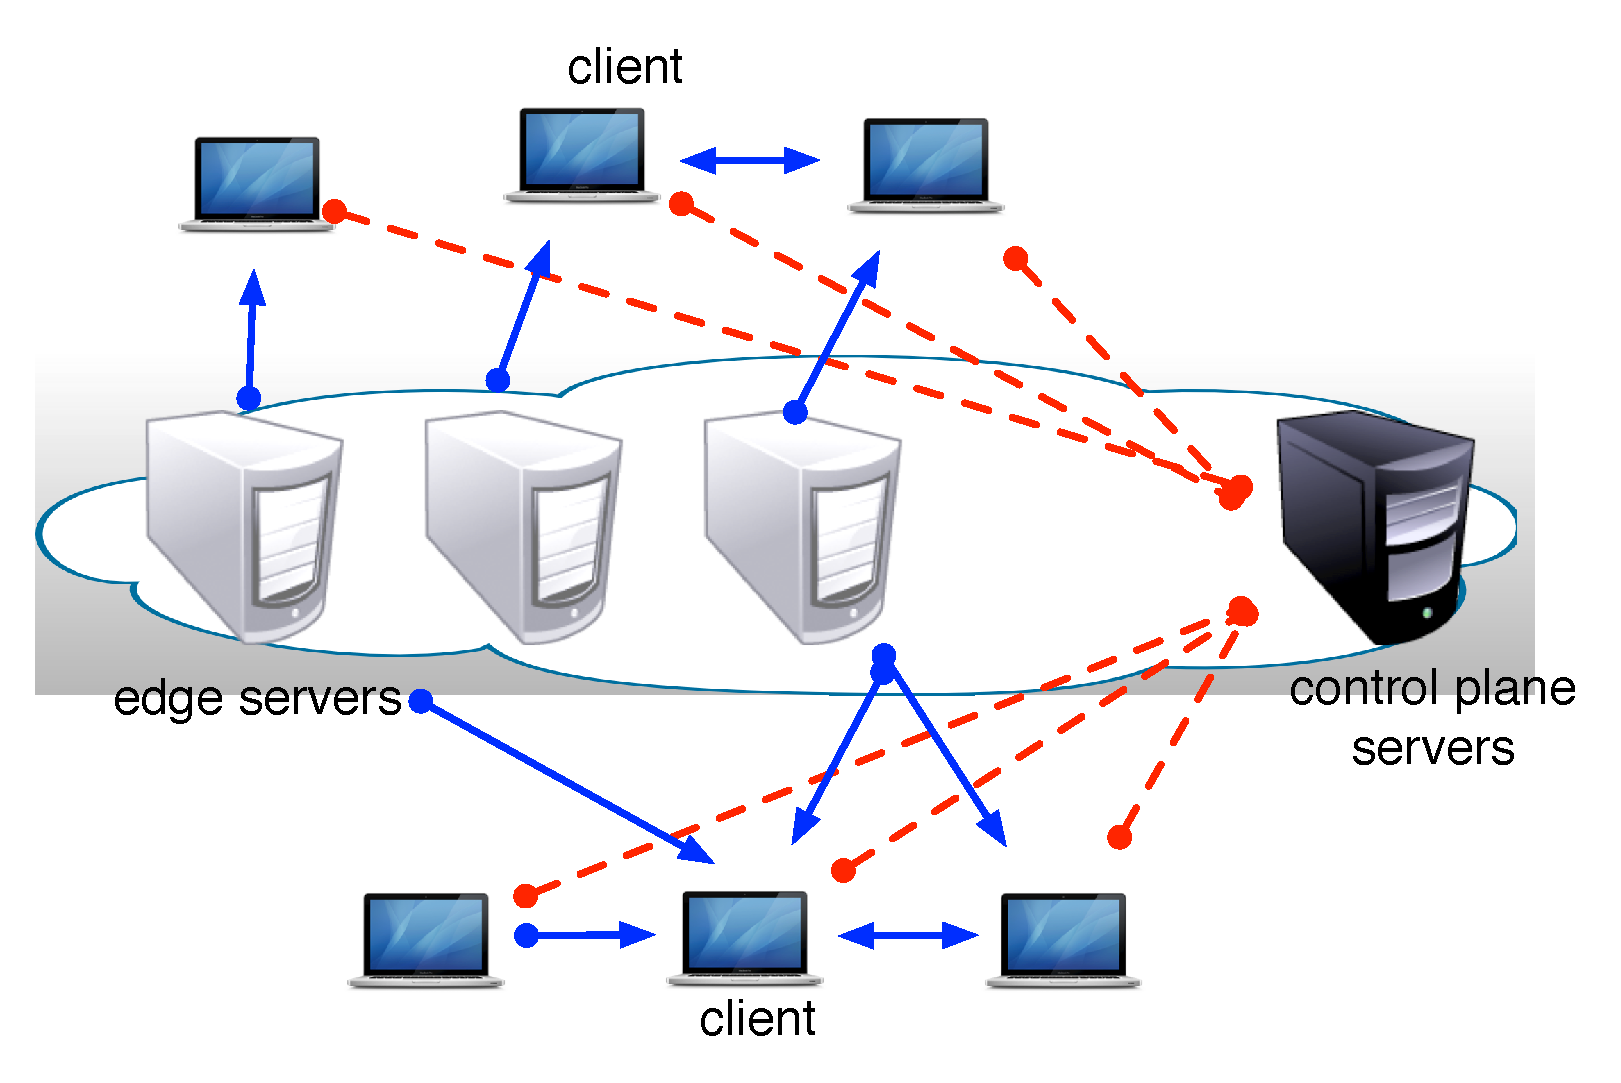
\includegraphics[scale=0.3]{graphs/netsession.eps}
%\end{center}
%\caption{Peer Assisted CDN Overview.}
%\label{fig:p2pcdnoverview}
%\end{figure} 




\section{Related Work}\label{relatedwork}
Content Distribution Networks with peer assist have been successfully deployed on the Internet, such as Akamai \cite{Zhao:2013:PCD:2504730.2504752}, \cite{Huang:2008:UHC:1496046.1496064} and LiveSky \cite{Yin:2010:LEC:1823746.1823750}.  
The authors of \cite{Zhao:2013:PCD:2504730.2504752} examine the risks and benefits of peer-assisted content distribution in Akamai and measure the effectiveness of its peer-assisted approach. 
The authors of \cite{Huang:2008:UHC:1496046.1496064} conclude from two real world traces that hybrid CDN-P2P can significantly reduce the cost of content distribution and can scale to cope with the exponential growth of Internet video content.  
Yin et al. \cite{Yin:2010:LEC:1823746.1823750} described commercial operation of a peer-assisted CDN in China.  
LiveSky solved several challenges in the system design, such as dynamic resource scaling of P2P, low startup latency, ease of P2P integration with the existing CDN infrastructure, and network friendliness and upload fairness in the P2P operation.  
Xu et al.\cite{DBLP:journals/corr/abs-1212-4915} used game-theory to show the right cooperative profit distribution of P2P can help the ISP to maximize the utility.  
Their model can easily be implemented in the context of current Internet economic settlements.  
Misra et al.\cite{Misra:2010:IPS:1811099.1811064} also mentioned the importance of P2P architecture to support content delivery networks.
The authors use cooperative game theory to formulate simple compensation rules for users who run P2P to support content delivery networks.

The idea of telco- or ISP-managed CDN has been proposed in recent years.  
The complexity of the CDN business encourage telcos and ISPs to manage their own CDN, rather than allow others to run CDNs on their networks.  
It has been shown that it is cost effective \cite{federation}\cite{norton2011internet}. 
Kamiyama et al. \cite{NoriakiKAMIYAMA2013} proposed optimally ISP operated CDN.
Kamiyama et al. mentioned that, in order to deliver large and rich Internet content to users, ISPs need to put their CDNs in data centers.  
The locations are limited while the storage is large, making this solution effective, using optimum placement algorithm based on real ISP network topologies.  
The authors found that inserting a CDN into an ISP's ladder-type network is effective in reducing the hop count, thus reduce total link cost.  
Based on the author definition: Ladder-type network is a network with a maximum degree under $10$.
Cisco has initiated an effort to connect telco- or ISP-managed CDNs to each other, to form a CDN federation \cite{federation} using open standards \cite{cdni}.  
They argue that the current CDN architecture is not close enough to the users and ISPs can fill this position.

The idea of utilizing the user's computation power to support ISP operation is not new.  
The Figaro project \cite{figaro} proposed the residential gateway as an integrator of different networks and services, becoming an Internet-wide distributed content management for a proposed future Internet architecture \cite{figaro}.  
Cha et al.,\cite{Cha:2008:NTP:1855641.1855646} performed trace analysis and found that an IPTV architecture powered by P2P can handle a much larger number of channels, with lower demand for infrastructure compared to IP multicast.  
Jiang et al. \cite{Jiang:2012:OMD:2413176.2413193} proposed scalable and adaptive content replication and request routing for CDN servers located in users' home gateways.  
Maki et al.,\cite{NaoyaMAKI2012} propose traffic engineering for peer-assisted CDN to control the behavior of clients, and present a solution for optimizing the selection of content files.
Mathieu et al., \cite{6249305} are using data gathered from France telecom network to calculate reduction of network load if customers are employed as peer-assisted content delivery.

Guo et al., \cite{1613869} work's PROP is closest with our work.
%because we use that work as comparison and we use author's utility function.
PROP uses local system (local counter) to calculate the segment popularity in peer-assisted proxy system. 
PROP uses popularity for proxy cache replacement strategy. 
In peer side, the author use utility function for cache replacement strategy.
A utility function assigns numerical value to outcomes, in such a way that outcomes with higher utility are always preferred ot outcomes with lower utilities.
The utility function is also function from popularity.
While the authors successfully show that the results are very good, the peer-assisted system behavior over time is not explain because the author focus on properties such as proxy cache size variations and peer cache size variations.
The explanation of the optimal number of replicas is not also clear because unavailable information when the snapshot is taken.  
In our work, we complement Guo et al., \cite{1613869} work with VoD viewing popularity evolution model and describe the behavior of the peer-assisted CDN over the time.

\begin{figure}[!t]
\begin{center}
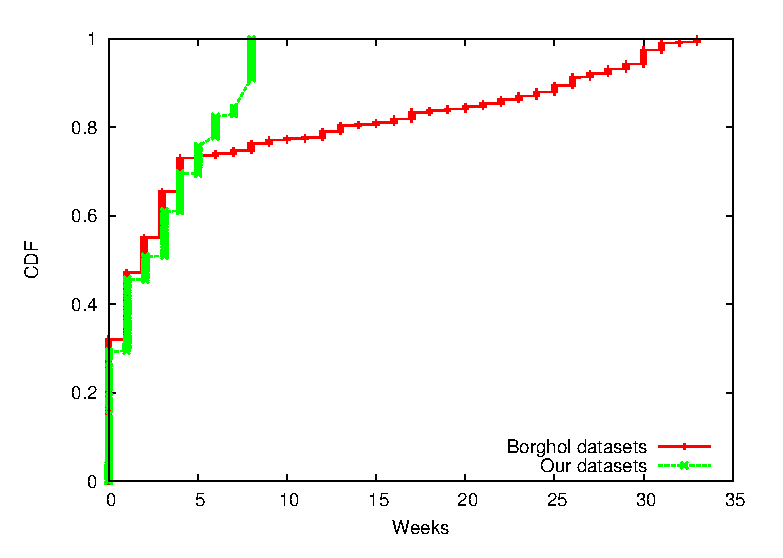
\includegraphics[scale=0.6]{graphs/timetopeak.eps}
\end{center}
\caption{Time to peak empirical distribution.}
\label{fig:timetopeak}
\end{figure} 

\section{Characterizing Internet VoD Popularity}\label{popularity}
Before analyzing the system description and video caching, we first examine the popularity characteristics of Internet VoD services.
We use YouTube as example of VoD service.
The studies of content popularity evolution are mostly considered in short time periods.
Borghol et al., \cite{Borghol:2011:CMP:2039452.2039717} measure the evolution of content popularity in long periods (36 weeks,from 3 August 2008 until 29 March 2009) in which view count statistics of Youtube. 

In datasets, we have one-week spacing between consecutive snapshots.  
We can get how many times the video was view during the one-week period since last week or since snapshot $(i-1)$. 
Borghol et al., \cite{Borghol:2011:CMP:2039452.2039717} define time-to-peak for a video as its age (time since upload) at which its weekly viewing rate is the highest during measurement (from the first week until end of measurement).

The time-to-peak distributions is shown in fig.\ref{fig:timetopeak}.
Figure \ref{fig:timetopeak} shows Borghol et al., \cite{Borghol:2011:CMP:2039452.2039717} work that around three-quarters of a large fraction videos peak within the first six weeks since their upload and beyond six weeks we have uniform distribution thus the time-to-peak is exponentially distributed mixture with uniform distribution. 
Because we know the peak time (at-peak phase) of every video, we can also know before-peak phase and after-phase of every videos.

To estimate the the rate parameter of exponential part of time-to-peak distribution, we use Maximum Likelihood Estimation (MLE) \cite{clauset2009power}.
Using MLE method, we can get exponential parameter $\lambda = 0.59$.
For weekly views distribution, Borghol et al., \cite{Borghol:2011:CMP:2039452.2039717} found that beta distribution is a good model to explain video views popularity evolution thus we follow Borghol et al., \cite{Borghol:2011:CMP:2039452.2039717} for  weekly views distribution model.\\
To reveal data distribution of view rate for every video, we plot view rate versus week where we shift week of view rate at-peak phase to zero. 
Therefore we can get view rate distribution relative to at-peak week as shown in fig.~\ref{fig:viewratedistribution}

\begin{figure}[!t]
\begin{center}
\includegraphics[scale=0.6]{graphs/datadistribution.eps}
\end{center}
\caption{View rate distribution versus week relative to at-peak phase week for every videos, where y-axis in logscale.
Every points lie in negative x-axis mean view rate of every videos in before-peak phase.
Every points lie in x-axis$=0$ mean view rate of every videos at-peak phase. 
Every points lie in positive x-axis mean view rate of every videos in after-peak phase. }
\label{fig:viewratedistribution}
\end{figure} 


\begin{figure}[!t]
\begin{center}
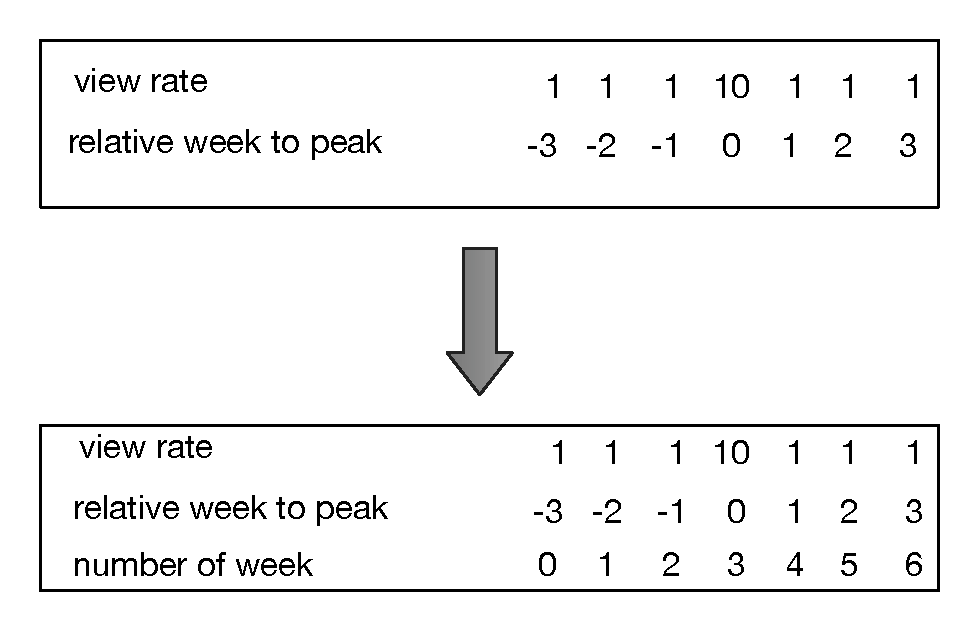
\includegraphics[scale=0.5]{graphs/transformasi.eps}
\end{center}
\caption{Transformation of view rate distribution. We add number week and make it as $x$-axis, View rate as $y$-axis, and relative week to peak as $z$-axis.}
\label{fig:viewratedistexample}
\end{figure} 

\begin{figure}[!t]
\begin{center}
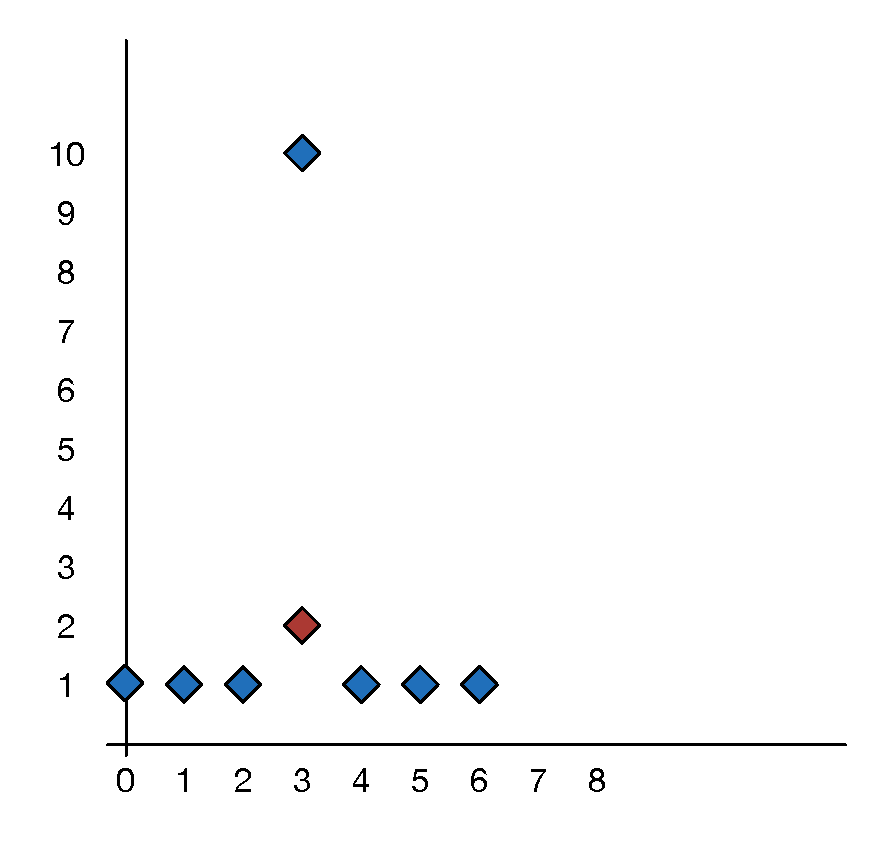
\includegraphics[scale=0.5]{graphs/transformasi2.eps}
\end{center}
\caption{Final view rate distribution after transformation where $x$-axis is number of week, $y$-axis is view rate.}
\label{fig:viewratedistexamplered}
\end{figure} 



\section{System Description}\label{systemdescription}
In our work, we use Youtube VoD view model to aid our work that based from PROP. 
The Youtube VoD view model will be used in peer-caching strategy side to exploits the video popularity. 


\subsection{Peer caching strategy}\label{peercachingstrategy}
As we mentioned before, we use Youtube VoD view model in peer caching strategy side. 
Our utility function is different from PROP.
Our utility function need the estimation of video position whether the requested video is in before-peak phase, at-peak phase, or after-peak phase.
How we estimate the video position is shown in fig.~\ref{fig:viewratedistexample} and fig.~\ref{fig:viewratedistexamplered}.
In fig.~\ref{fig:viewratedistexample} part A, we have view rate (y-axis) and relative week to peak (x-axis) which is view rate distribution versus week relative to at-peak phase as also shown completely in fig.~\ref{fig:viewratedistribution}.
We transform these numbers by adding number of week and make number of week as x-axis, view rate 
as y-axis, and relative week to peak as z-axis fig.~\ref{fig:viewratedistexample} part B.
This transformation is shown in fig.~\ref{fig:viewratedistexamplered} as diamond points.
We want to estimate what is the position of that video. 
Is the video in at-peak phase, before-phase, or after phase.  
We can estimate the that video position by averaging relative week to peak numbers (the points at z-axis) of the nearest point from datasets. 
If the average value less than $0$ we estimate the video position at before-peak phase, if the average value equal to $0$ we estimate the video position at at-peak phase,  and if the average value more than $0$ we estimate the video position at after-peak phase.

For example: there is a peer that request a video where the position of video in third week with the last week view rate $vr=2$ (we can get as this data from CDN) shown in fig.~\ref{fig:viewratedistexamplered} as red cross.
In this case, the nearest points are the point at third week $(2,1,-1)$ and the point at fifth week $(4,1,1)$.  
By averaging the points at z-axis of the nearest points $(-1 + 1)/2 = 0$,  we can get estimate that video is in at-peak phase.

Since we can estimate before-peak week, at-peak week, and after-peak week of video, we modified the original utility function from PROP by adding a weight as follows:
\begin{equation}
u = \frac{ (f(p) - f(p_{min})) (f(p_{max}) - f(p)) }{r^{\alpha + \beta}} + weight
\end{equation}
where $weight$ is proportion of view count that we get from Youtube datasets.  
In before-peak week, we get $weight=0.149538787758 $,  in at-peak week, we get $weight=0.470040393021$, and in after-peak week, we get $weight=0.380420819221$.
$p$ represents popularity of the video, $p_{min}$ represents estimation of minimum popularity in P2P system, $p_{max}$ represents estimation of maximum popularity in P2P system, $r$ represents the number of replicas of the video in the system, and $f(p)$ is monotonic non-decreasing function.
$\alpha$ and $\beta$ are the adjustment factor.
The CDN can calculate $p_{min}$ and $p_{max}$ then propagate to the P2P system.
To able to track the simulation, we use default value from PROP for $\alpha=\beta=1$ and $f(p)=log (p)$.
We choose the video with the smallest $u$ value as the candidate to be replaced when a peer's cache capacity is full.

\begin{figure}[!t]
\begin{center}
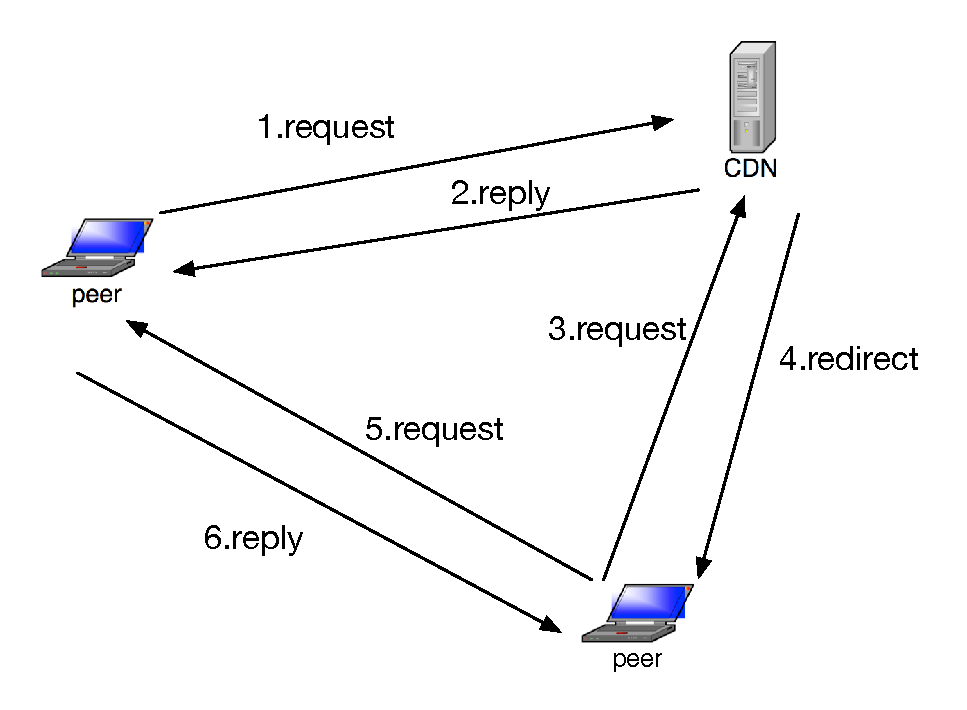
\includegraphics[scale=0.4]{graphs/p2p-system-description.eps}
\end{center}
\caption{Peer interaction in simulator.}
\label{fig:p2pcdninteractioninsimulator}
\end{figure} 



\section{Evaluation}\label{evaluation}
%apa yng dievaluasi.
%bandingkan 2 proposal ini dng 2 metric yng ada misalnya.
%kenapa 2 metric ini dipilih.
%bagaimana evaluasinya:  bikin simulator: a, b, c ,d 

In order to evaluate the proposed peer-caching strategy using before-peak, at-peak, and after-peak information from Youtube VoD view model, we have to compare our model to PROP model.
We evaluate three metrics which are peer contribution to delivery contents during simulation,  access frequency of cache during simulation, and number of replicas. 
Peer contribution metric related to byte-hit-ratio. 
Byte-hit-ratio is defined as the total bytes contents served by peers normalized by the total bytes of video all peers and CDN consume.
It means more peer contributions, more byte-hit-ratio because peer can get content from another peers. 
Access frequency of cache reflects the storage utilization. 
More access means more peer storage utilization.  
Number of replicas is also related to peer storage utilization.  
How ever, too many replicas will waste the storage resources.
To evaluate these metrics, we developed a peer-assisted CDN simulator. 


\subsection{Simulation Design}\label{simulationdesign}
An event driven simulator is developed using Python for this purpose.
In our simulator, time is divided into rounds. 
During a round, a peer request a video.

In fig.\ref{fig:p2pcdninteractioninsimulator}, we describe the process of a peer that requests a video in simulator which derived from PROP.
A peer and a CDN are implemented in object oriented model. 
When a peer requests a video, it always goes to a CDN server (step 1). 
The CDN provides the videos to the peer (step 2). 
If there is another peer request same video, that request will go to CDN (step 3).  
A CDN will check its record to see if there are some peers cache that requested video.  
If there are some peers cache that requested video, a CDN will reply with redirect message that asking a peer to download requested video from other peer (step 4).
If there are no peers have requested video, a CDN will serve the video.   
A peer then can request the video to other peer and get the video (step 5 and step 6).
From above description, we can see that deploying peer-assisted CDN can save some traffic since the clients which form P2P network can sharing the contents or videos.


\subsubsection{Catalog Generator}\label{catalog}
The goal for catalog generator is to create a catalog video that consist video-id, time when a video is uploaded, a video size, and view count terminus.
We made catalog that consists of 10000 videos thus we have video-id from 0 until 9999.
We assume that a video is uploaded to server following poisson process with mean rate $\lambda=1$ thus we can get the time when a video is uploaded. 
The view count terminus for every video is assigned randomly from Youtube datasets and video size for every video is assigned randomly between $1$MB and $200$MB. 

In last step, we assign file size of video randomly between $1$MB and $200$MB.
Finally, we have a catalog that consists of: video-id, time when a video is uploaded, view count terminus, and video size.



\subsubsection{Peer Request Generator}\label{peerrequest}
In catalog generator, we assume peer request a video to CDN following poisson process with a mean rate $\lambda=1$ \cite{Zink:2009:CYN:1502814.1502987} %and we made it 3600 videos per hour, 
finally we generate video request for 360 days of simulation.

We assume that a peer choose a video based on a preference from view count and view rate.
First, we calculate the number of videos at-peak time as follows: sample $N$ value from the time-to-peak distribution and determine the number of videos $n_j^{at}$ that peak at week $j$. 
Total number of video $N = n_j^{before} + n_j^{at} + n_j^{after}$.\\
Next, we determine view count terminus which are the number of final view count of video.
In view count terminus, we assume that a video will not get big additional view after at-peak phase.
We assign view count terminus randomly from datasets.
After determining view count terminus, we assign beta distribution parameter for every video. 
Since we can estimate the time of at-peak phase for each video, we know the mode of beta distribution value and we can calculate $\alpha$ and $\beta$ value using the mode of distribution formula: $m=\frac{\alpha-1}{\alpha + \beta - 2}$.  
We assign $\alpha$ value randomly between $1$ and $2$ thus we can calculate $\beta$ value.
With the knowledge of beta distribution of every video and its view count terminus, we can know the view count and view rate of every video as function from time.
The knowledge of view count and view rate, will be used top generate a video choice that used by a peer.  
For video choice, we estimate that a peer will choose video proportionally considering view count and view rate of the video.   
We can get view count and view rate from probability distribution function (PDF) and cumulative distribution function (CDF) of beta distribution above multiply by video's view count terminus.
Finaly, we have requests catalog that consists of: peer-id, request time, and video-id to be choosen.

\subsubsection{Simulation Parameters and Scenarios}
The simulation parameters are follows:
\begin{itemize}
\item Length: $360$ days.
\item Video size: random between $1$MB and $200$MB.
\item Peer capacity: [500MB].
\item CDN capacity: $10000$MB.
\item Number of peers: $100000$.
\item Number of videos: $10000$.
\end{itemize}
We compare our results to original PROP \cite{1613869} implementation.
There are three scenarios in our simulations.
First, peers choose a video that has a popularity following from Youtube data sets that we already explained in \ref{catalog}.
Second, peers choose a video that has a popularity following from Youtube data sets and we shift the requests time four weeks.
Third, peers choose a video that has a popularity following zipf distribution with rate$=0.9$ \cite{6654887}.





%%%%%%%%%%%%%%%%%%%%%%%%% FIGURE %%%%%%%%%%%%%%%%%%%%%%%%%%%%%%%%%%%
%%%contribution 
\begin{figure*}[!t]
\centering
\subfloat[Absolute of contribution of peer for the first scenario.\label{fig:contribu-normal}]{
\includegraphics[width=5.7cm]{graphs/new/repl/contributioncdnpeermodelsortedabs.png}
}
\hfill
\subfloat[Absolute of contribution of peer for the second scenario.\label{fig:contribu-shift}]{
\includegraphics[width=5.7cm]{graphs/new/shift/contributioncdnpeermodelsortedabs.png}
}
\hfill
\subfloat[Absolute contribution of peers for the third scenario.\label{fig:contrib-zipf}]{
\includegraphics[width=5.7cm]{graphs/new/zipf/contributioncdnpeermodelsortedabs.png}
}
\vspace{2mm}
\caption{Peer contributions compared between model and prop.}
\label{fig:peercontribution}
\end{figure*}
%%%%%%%%%%%%%%%%%%%%%%%%%% FIGURE %%%%%%%%%%%%%%%%%%%%%%%%%%%%%%%%%%%



\subsection{Result and Discussion}\label{resultanddiscussion}
Figure \ref{fig:contribu-normal}, \ref{fig:contribu-shift}, and \ref{fig:contrib-zipf} show the absolute peer contribution to deliver videos compared between model and prop. 
Figure \ref{fig:contribu-normal} and fig.\ref{fig:contribu-shift} show same pattern.
The peers give more contribution in the tail while in the third scenario the peer give more contribution in body. 
A peers can give more contribution because a video has longer duration than other videos in a peer's cache thus other peer's requests are served by the peer. 
A video has longer duration than other videos in peer's cache because that a video has bigger utility function than other videos for example a video that will enter the cache. 

Denote $u_{dl}$ is utility function for a video inside the cache and $u_{ms}$ is utility function for a video that will enter the cache,  $p_{dl}$ is the popularity for a video inside the cache and $p_{ms}$ is the popularity for a video that will enter the cache.
In order a video in cache has longer duration, the utility function for $u_{dl}$ must be bigger than the utility function for $u_{ms}$.
\begin{equation*}
u_{dl} > u_{ms}
\end{equation*}

\begin{align*}
\frac{ (f(p_{dl}) - f(p_{min})) (f(p_{max}) - f(p_{dl})) }{r^{\alpha + \beta}_{dl}} + weight_{dl} > \\
\frac{ (f(p_{ms}) - f(p_{min})) (f(p_{max}) - f(p_{ms})) }{r^{\alpha + \beta}_{ms}} + weight_{ms}
\end{align*}
We assume that number of replicas are same, thus:
\begin{align*}
(f(p_{dl}) - f(p_{min})) (f(p_{max}) - f(p_{dl})) - \\ 
(f(p_{ms}) - f(p_{min})) (f(p_{max}) - f(p_{ms})) > \\
weight_{ms} - weight_{dl}
\end{align*}
Since $p_{min}$ and $p_{max}$ are same, we can find that the difference between $p_{dl}$ and $p_{ms}$ must always bigger than the difference between $weight_{ms}$ and $weight_{dl}$.
If both videos are in the same position (e.g before-peak, at-peak, or after-peak) then the video popularity is the only factor. 
However, if the videos are not in the same position then the difference between $p_{dl}$ and $p_{ms}$ must always bigger than the difference between $weight_{ms}$ and $weight_{dl}$.
There are two cases for the difference between $weight_{ms}$ and $weight_{dl}$.
The first case is negative and the second case is positive.  
Since we only interested in positive case, we will explain the positive case.  










%%%%%%%%%%%%%%%%%%%%%%%%% FIGURE %%%%%%%%%%%%%%%%%%%%%%%%%%%%%%%%%%%
%%%freq
\begin{figure*}[!t]
\centering
\subfloat[Frequency a video in peers for the first scenario.\label{fig:freq-normal}]{
\includegraphics[width=5.7cm]{graphs/new/repl/freq.png}
}
\hfill
\subfloat[Frequency a video in peers for the second scenario.\label{fig:freq-shift}]{
\includegraphics[width=5.7cm]{graphs/new/shift/freq.png}
}
\hfill
\subfloat[Frequency a video in peers for the third scenario.\label{fig:freq-zipf}]{
\includegraphics[width=5.7cm]{graphs/new/zipf/freq.png}
}
\vspace{2mm}
\caption{Frequency a video in peers compared between model and prop.}
\label{fig:freq}
\end{figure*}
%%%%%%%%%%%%%%%%%%%%%%%%%% FIGURE %%%%%%%%%%%%%%%%%%%%%%%%%%%%%%%%%%%



%%%%%%%%%%%%%%%%%%%%%%%%% FIGURE %%%%%%%%%%%%%%%%%%%%%%%%%%%%%%%%%%%
%%%duration
\begin{figure*}[!t]
\centering
\subfloat[Cache duration in peers for the first scenario.\label{fig:duration-normal}]{
\includegraphics[width=5.7cm]{graphs/new/repl/duration.png}
}
\hfill
\subfloat[Cache duration in peers for the second scenario.\label{fig:duration-shift}]{
\includegraphics[width=5.7cm]{graphs/new/shift/duration.png}
}
\hfill
\subfloat[Cache duration in peers for the third scenario.\label{fig:duration-zipf}]{
\includegraphics[width=5.7cm]{graphs/new/zipf/duration.png}
}
\vspace{2mm}
\caption{Duration compared between model and prop.}
\label{fig:duration}
\end{figure*}
%%%%%%%%%%%%%%%%%%%%%%%%%% FIGURE %%%%%%%%%%%%%%%%%%%%%%%%%%%%%%%%%%%


%%%%%%%%%%%%%%%%%%%%%%%%% FIGURE %%%%%%%%%%%%%%%%%%%%%%%%%%%%%%%%%%%
%%%replica
\begin{figure*}[!t]
\centering
\subfloat[Number of a video replicas when a peer request a video for the first scenario.\label{fig:atd-normal}]{
\includegraphics[width=5.7cm]{graphs/new/repl/atd.png}
}
\hfill
\subfloat[Number of a video replicas when a peer request a video for the second scenario.\label{fig:atd-shift}]{
\includegraphics[width=5.7cm]{graphs/new/repl/atd.png}
}
\hfill
\subfloat[Number of a video replicas when a peer request a video for the third scenario where $y$ axis in log-scale.\label{fig:atd-zipf}]{
\includegraphics[width=5.7cm]{graphs/new/zipf/atd.png}
}
\vspace{2mm}
\caption{Replicas compared between model and prop.}
\label{fig:replica}
\end{figure*}
%%%%%%%%%%%%%%%%%%%%%%%%%% FIGURE %%%%%%%%%%%%%%%%%%%%%%%%%%%%%%%%%%%











\section{Conclusion and Future Work}\label{conclusion}
This paper presents a scheme for a ISP managed peer-assisted CDN model that 
Some areas of improvement that we have identified for future are:
We are also very interested to include energy trade off this peer-assisted CDN architecture in order to know how much energy saving by ISP and how much increase of energy at users home gateway side in this architecture.


% use section* for acknowledgement
\section*{Acknowledgment}
The authors would like to thank Internet research laboratory member at Keio University and anonymous reviewers.





% trigger a \newpage just before the given reference
% number - used to balance the columns on the last page
% adjust value as needed - may need to be readjusted if
% the document is modified later
%\IEEEtriggeratref{8}
% The "triggered" command can be changed if desired:
%\IEEEtriggercmd{\enlargethispage{-5in}}

% references section

% can use a bibliography generated by BibTeX as a .bbl file
% BibTeX documentation can be easily obtained at:
% http://www.ctan.org/tex-archive/biblio/bibtex/contrib/doc/
% The IEEEtran BibTeX style support page is at:
% http://www.michaelshell.org/tex/ieeetran/bibtex/
%\bibliographystyle{IEEEtran}
% argument is your BibTeX string definitions and bibliography database(s)
%\bibliography{IEEEabrv,../bib/paper}
%
% <OR> manually copy in the resultant .bbl file
% set second argument of \begin to the number of references
% (used to reserve space for the reference number labels box)
\bibliographystyle{IEEEtran}
\bibliography{manu}

% that's all folks
\end{document}


